\documentclass[journal]{IEEEtran}

\usepackage{graphicx}
\usepackage{amsmath}
\usepackage{url}
\usepackage{array}
\usepackage{tabularx}

\graphicspath{{images/}}

% Define a clean, clickable hyperlink macro using pdfTeX primitives
\newcommand{\hrefgh}[2]{%
  \leavevmode\pdfstartlink user{/Subtype /Link /A << /S /URI /URI (#1) >>}%
  #2%
  \pdfendlink%
}

\title{Analysis and Classification of Physical Actions Using Surface Electromyography (sEMG) Signals}

\author{
    \IEEEauthorblockN{Academic Course Project Report} \\
    \IEEEauthorblockA{Analysis of Physical Actions Using EMG Signal Classification}
}

\begin{document}

\maketitle

% First page GitHub repository callout box with icon
\begin{center}
\fbox{%
  \parbox{0.95\columnwidth}{%
    \centering\footnotesize
    \hrefgh{https://github.com/WebProject05/EMG_PhysicalSignal_Analysis}{%
      \raisebox{-0.25ex}{
\includegraphics[height=1.15em]{github_icon.png}}~\textbf{Project Code \& Data on GitHub:}\\
      \texttt{https://github.com/WebProject05/EMG\_PhysicalSignal\_Analysis}%
    }%
  }%
}
\end{center}
\vspace{0.8em}

\begin{abstract}
Surface electromyography (sEMG) measures the electrical activity that muscles produce when they contract. In this project, we analyze an 8-channel sEMG dataset to classify different human physical actions. The dataset contains recordings from 4 subjects performing 20 different actions, split evenly into 10 normal daily activities (such as walking, standing, and waving) and 10 aggressive actions (such as punching, kicking, and elbowing), with 15 trials per action for a total of 1,200 trials. We extract statistical features by dividing each trial into four time segments and computing the mean and standard deviation for each channel, creating a 64-dimensional feature vector. We then use a $k$-Nearest Neighbors ($k$-NN) classifier inside a leakage-free standardization pipeline with 5-fold cross-validation. In binary classification between normal and aggressive actions, the model achieves an accuracy of 84.08\% (with an optimal $k=1$ achieving 85.50\%) and an AUC of 0.91. For multiclass classification, we study how accuracy decreases as the number of classes grows from $M=2$ to $M=19$ using Monte Carlo sampling across 10 random combinations per class count. The accuracy drops gradually from 83.83\% for 2 classes down to 35.73\% for 19 classes, remaining well above random chance. On the complete 20-class task, the system achieves 35.08\% accuracy compared to the 5\% random guessing level. All code and notebooks are publicly available in the linked GitHub repository.
\end{abstract}

\begin{IEEEkeywords}
Electromyography (sEMG), Physical Action Recognition, Feature Extraction, $k$-Nearest Neighbors, Classification Degradation, Machine Learning.
\end{IEEEkeywords}

\section{Motivation for the Classification Problem}
\IEEEPARstart{H}{uman} physical activity recognition has become an essential area of study across healthcare, sports science, robotics, and safety monitoring. Traditionally, human movements are tracked using optical cameras or wearable motion sensors like accelerometers and gyroscopes. However, optical cameras suffer from severe privacy concerns, can be obstructed by objects, and fail in low-light environments. Inertial measurement units (IMUs) measure movement only after the limbs have already begun moving through space, which limits their reaction speed.

Surface electromyography (sEMG) offers an attractive alternative. Because sEMG detects the electrical action potentials generated directly by contracting skeletal muscles, it captures the human motor intention at the neuromuscular level---often fractions of a second before noticeable movement occurs.

Automating the classification of physical actions using sEMG is motivated by several real-world applications:
\begin{itemize}
    \item \textbf{Smart Healthcare and Rehabilitation:} Physical therapists need objective data to evaluate whether patients recovering from orthopedic injuries or strokes are performing exercises correctly. Automatic action recognition provides a quantitative record of muscle engagement without needing continuous manual supervision.
    \item \textbf{Automated Safety and Threat Detection:} Detecting sudden aggressive behavior (such as punching, kicking, or elbowing) in elder-care facilities, mental health wards, or public safety environments can trigger emergency alarms while completely respecting privacy, as no video recording is involved.
    \item \textbf{Assistive Devices and Prosthetics:} Upper-limb and lower-limb amputees rely on intuitive control systems for powered prosthetics. Recognizing intended physical actions from residual muscle signals allows seamless, natural device operation.
    \item \textbf{Ergonomics and Sports Science:} Tracking fatigue and improper movement form during repetitive athletic actions helps prevent musculoskeletal injuries.
\end{itemize}

Given these motivations, developing a reliable and computationally lightweight machine learning framework that can classify both broad behavioral categories (normal vs. aggressive) and specific individual actions from muscle signals is highly valuable.

\section{Introduction to Physical Actions Classification Using Machine Learning Approaches}
Surface electromyography recordings present unique challenges for automated classification. Unlike clean laboratory signals, raw sEMG signals are non-stationary, stochastic, and look like random voltage fluctuations. Signal amplitude and timing vary widely depending on electrode positioning, skin moisture, subject muscle mass, and fatigue level.

To classify actions from sEMG data using machine learning, researchers typically follow a multi-step pattern recognition approach:
\begin{enumerate}
    \item \textbf{Signal Preprocessing and Windowing:} Continuous muscle recordings are partitioned into discrete movement trials or temporal windows to isolate active muscle contractions from background silence.
    \item \textbf{Feature Extraction:} Slicing the raw data into informative summary numbers. Instead of using raw voltage samples directly, statistical time-domain descriptors (such as mean, standard deviation, root-mean-square, or zero-crossings) or frequency-domain features are extracted. These reduce data dimensionality while retaining essential information about muscle contraction vigor and duration.
    \item \textbf{Supervised Classification:} Feeding the extracted feature vectors into supervised machine learning algorithms. Commonly used classifiers include $k$-Nearest Neighbors ($k$-NN), Support Vector Machines (SVM), Decision Trees, and Artificial Neural Networks.
\end{enumerate}

In this project, we implement a lightweight, interpretable classification framework using the $k$-Nearest Neighbors ($k$-NN) algorithm. The $k$-NN classifier is particularly well-suited for this task because it makes no rigid assumptions about the underlying data distribution and forms flexible decision boundaries based directly on Euclidean distance in feature space. To guarantee unbiased evaluation, feature standardization is encapsulated inside cross-validation loops to prevent data leakage.

\section{Block Diagram of the Proposed Classification Approach}
Fig.~\ref{fig:block_diagram} shows the complete pipeline of the proposed classification approach, illustrating the flow of data from raw muscle recordings to final classification decisions.

\begin{figure*}[t]
    \centering
    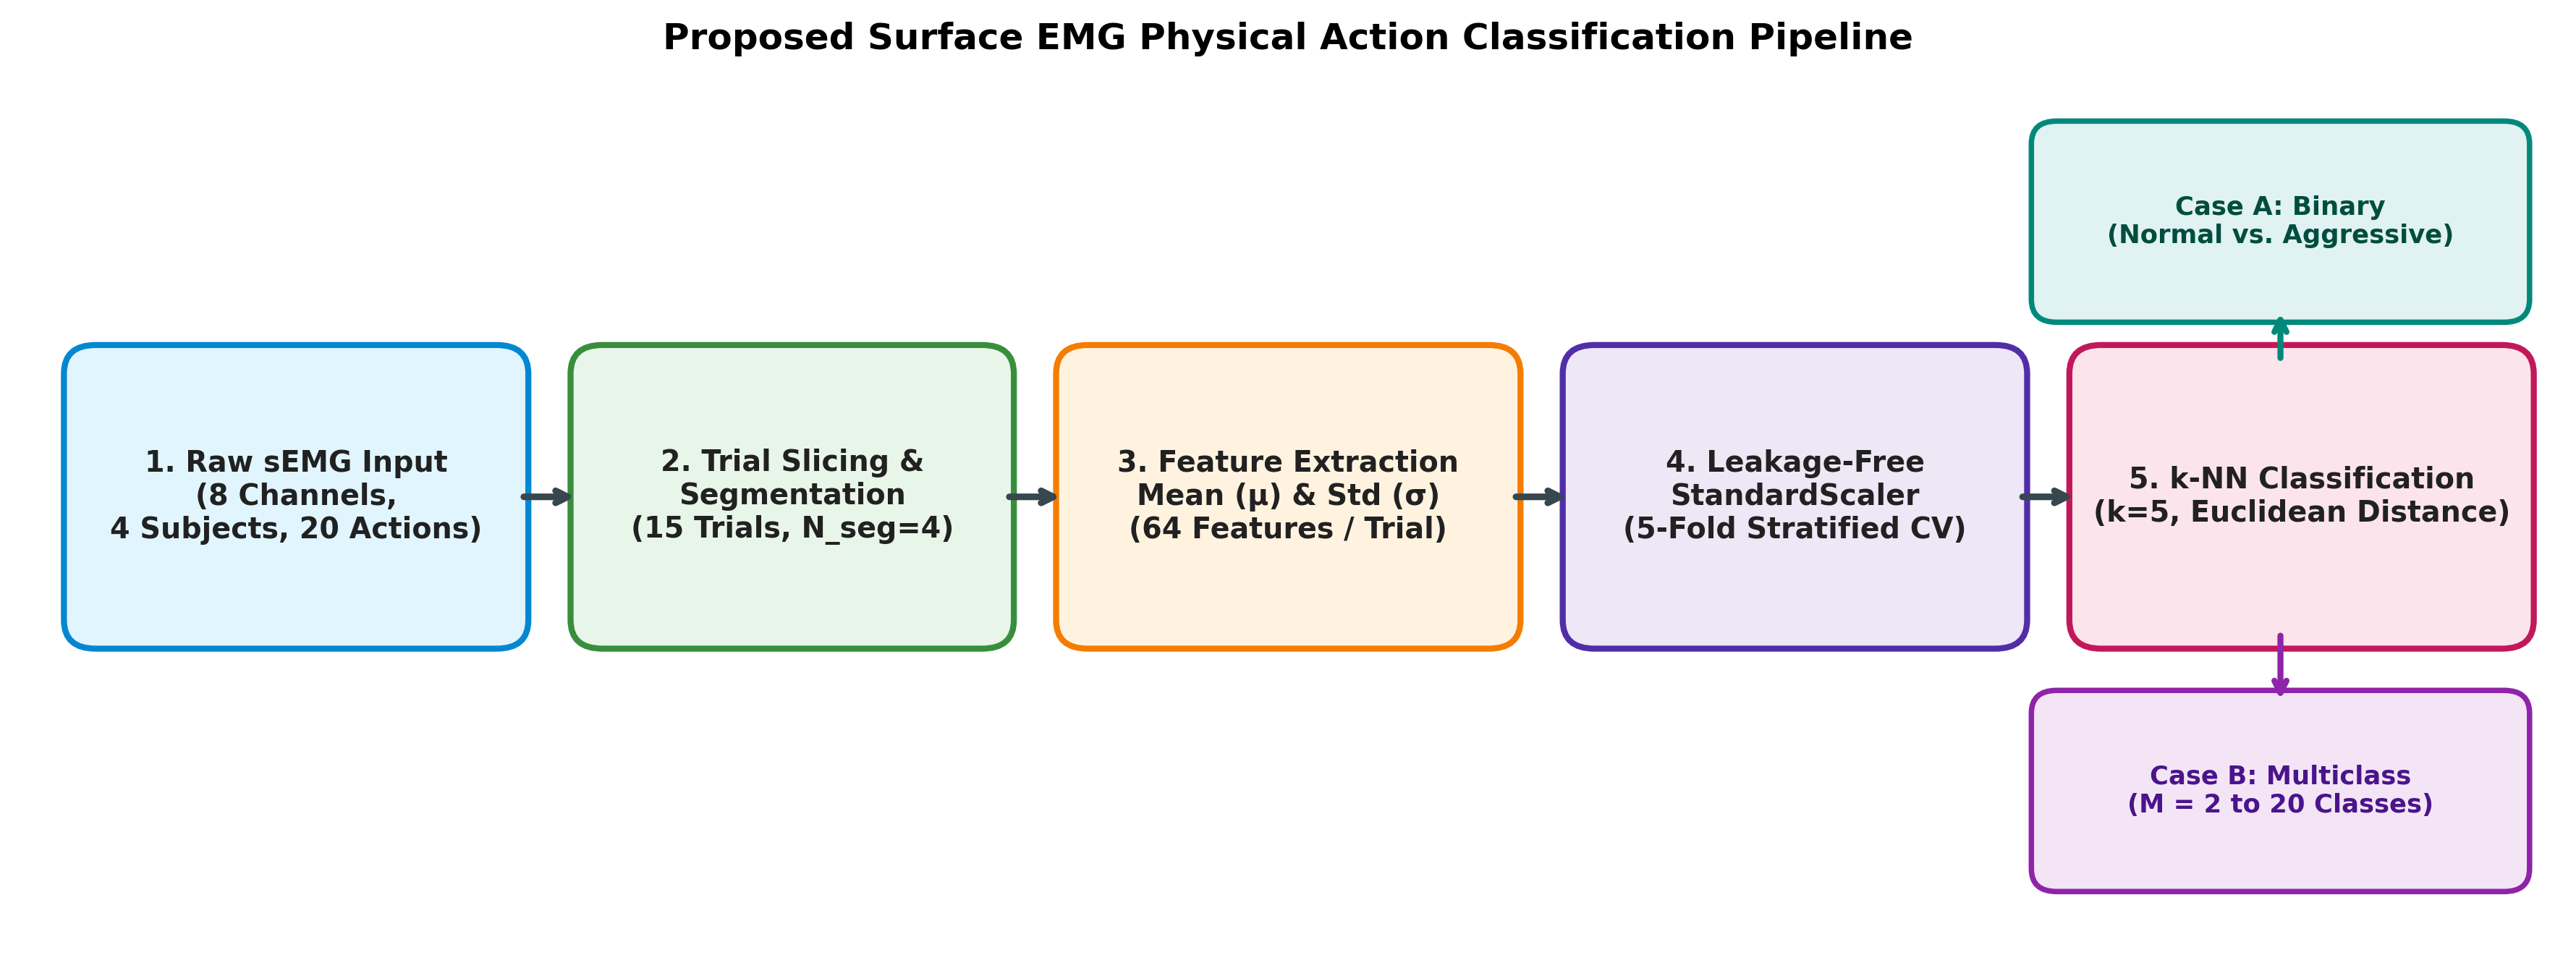
\includegraphics[width=0.92\textwidth]{00_proposed_pipeline_block_diagram.png}
    \caption{Block diagram of the proposed surface EMG physical action classification approach, showing raw data acquisition, trial slicing, temporal feature extraction, leakage-free standardization, and classification into binary and multiclass case studies.}
    \label{fig:block_diagram}
\end{figure*}

The pipeline consists of five key functional blocks:
\begin{enumerate}
    \item \textbf{Raw sEMG Input:} Continuous 8-channel recordings captured across 4 human subjects performing 20 physical actions.
    \item \textbf{Trial Slicing and Windowing:} Dividing each continuous action recording into 15 individual trials, and then partitioning each trial into 4 equal, non-overlapping temporal segments ($N_{seg} = 4$).
    \item \textbf{Feature Extraction:} Computing two statistical features---the Mean ($\mu$) and Standard Deviation ($\sigma$)---for each channel across each of the 4 segments, generating a compact 64-dimensional feature vector for each trial.
    \item \textbf{Leakage-Free Preprocessing:} Embedding feature standardization (\texttt{StandardScaler}) inside a scikit-learn \texttt{Pipeline} evaluated via 5-Fold Stratified Cross-Validation, ensuring test fold data never influences training statistics.
    \item \textbf{Classification Engine ($k$-NN):} Classifying the standardized feature vectors under two distinct experimental case studies:
    \begin{itemize}
        \item \textbf{Case Study A (Binary):} Distinguishing general Normal actions from Aggressive movements, as well as pairwise action discrimination.
        \item \textbf{Case Study B (Multiclass):} Evaluating performance degradation across subset sizes from $M=2$ to $M=19$ classes via Monte Carlo sampling, and benchmarking the complete 20-class classification task.
    \end{itemize}
\end{enumerate}

\section{Implementation of the Method on the Physical Actions Dataset}

\subsection{Short Description of the Dataset}
The project uses the benchmark \textit{EMG Physical Action Data Set}. Key characteristics of the dataset include:
\begin{itemize}
    \item \textbf{Subjects:} 4 healthy participants (\texttt{sub1}, \texttt{sub2}, \texttt{sub3}, \texttt{sub4}).
    \item \textbf{Sensors (8 Channels):} Electrodes placed on 8 major muscle locations:
    \begin{itemize}
        \item Right Biceps (CH1) and Right Triceps (CH2)
        \item Left Biceps (CH3) and Left Triceps (CH4)
        \item Right Thigh (CH5) and Right Hamstring (CH6)
        \item Left Thigh (CH7) and Left Hamstring (CH8)
    \end{itemize}
    \item \textbf{Actions (20 Classes):} 10 Normal daily actions (Bowing, Clapping, Handshaking, Hugging, Jumping, Running, Seating, Standing, Walking, Waving) and 10 Aggressive actions (Elbowing, Frontkicking, Hammering, Headering, Kneeing, Pulling, Punching, Pushing, Sidekicking, Slapping).
    \item \textbf{Trials:} Each recording contains 15 consecutive repetitions of the action. Total dataset size: $4 \times 20 \times 15 = 1,200$ trial samples.
\end{itemize}

\subsection{Visual Inspection of Raw Waveforms}
Fig.~\ref{fig:raw_bowing} and Fig.~\ref{fig:raw_punching} show the raw 8-channel signals for a representative normal action (Bowing) and aggressive action (Punching).

\begin{figure}[htbp]
    \centering
    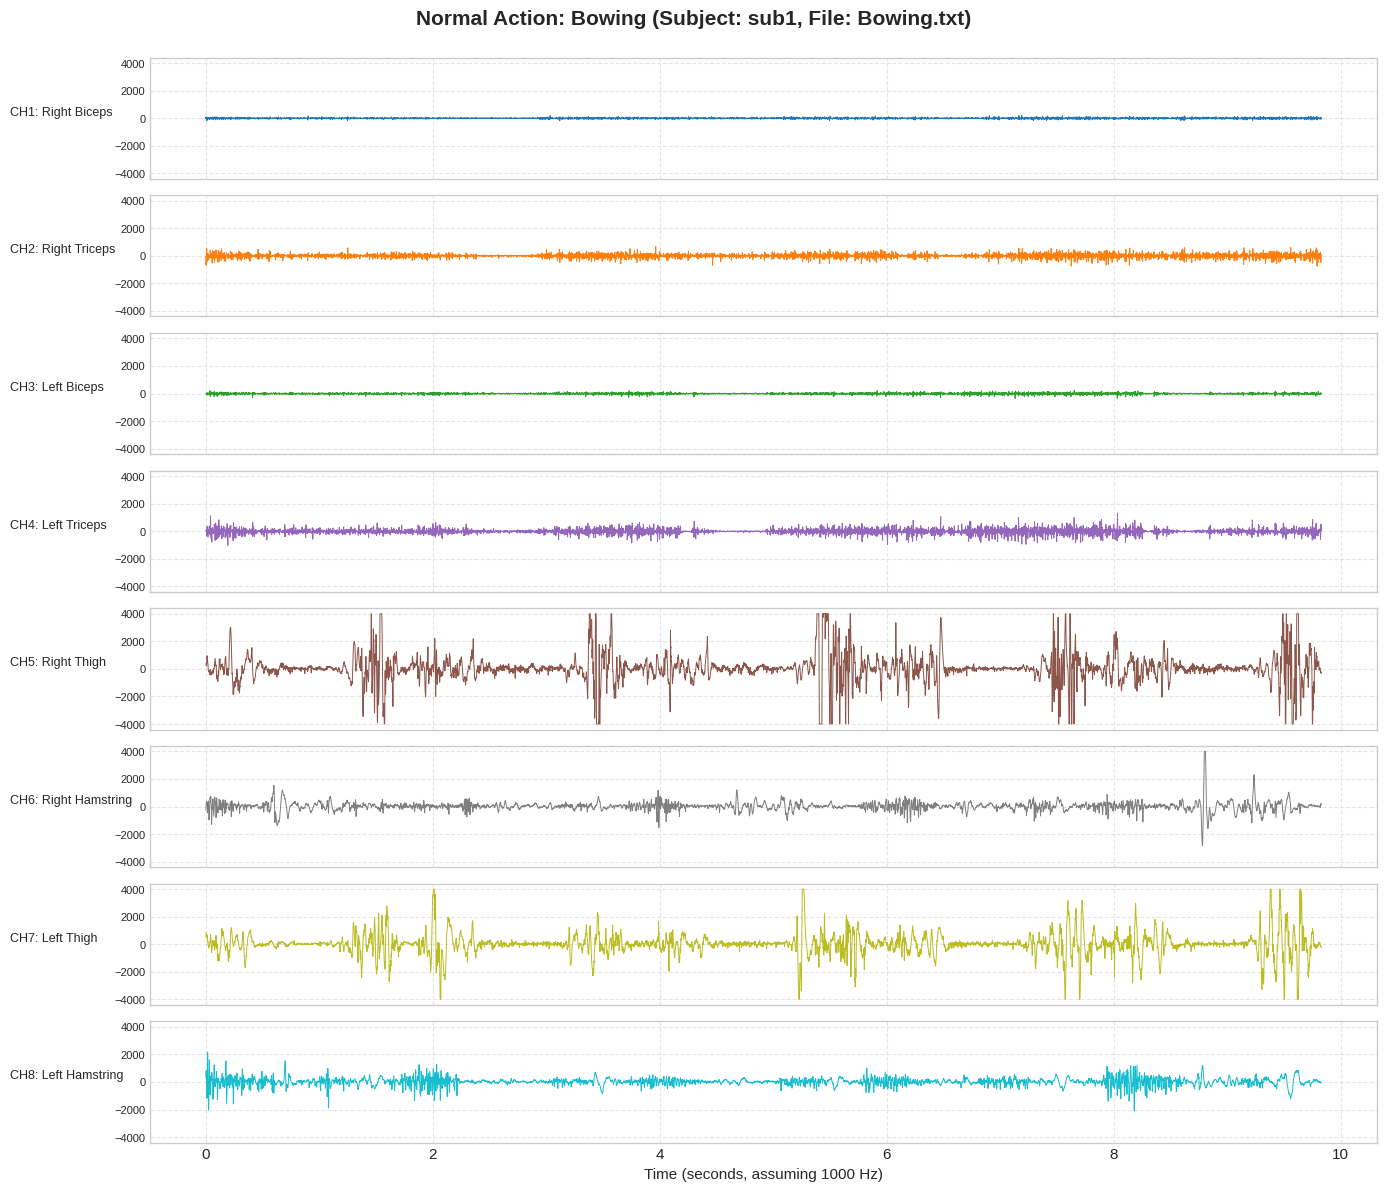
\includegraphics[width=\columnwidth]{01_normal_action_bowing_raw_emg.png}
    \caption{Raw 8-channel sEMG signals recorded during the normal action ``Bowing'' (Subject 1). Notice the smooth, steady electrical activity primarily concentrated on the leg channels (CH5--CH8).}
    \label{fig:raw_bowing}
\end{figure}

\begin{figure}[htbp]
    \centering
    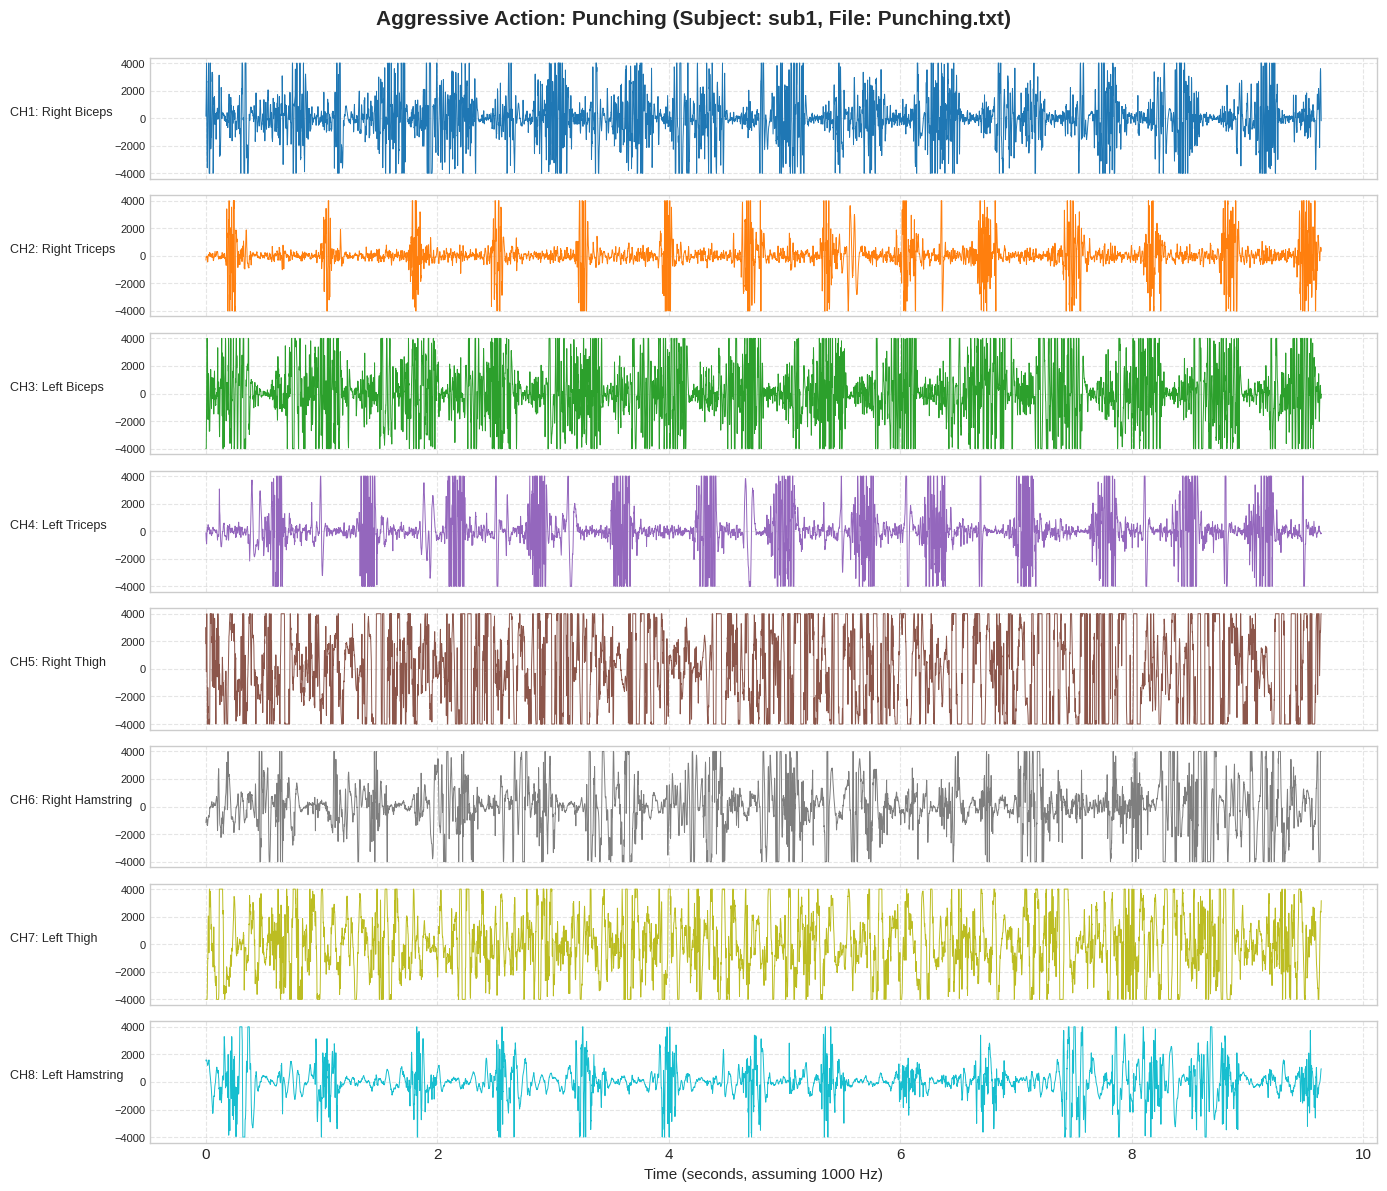
\includegraphics[width=\columnwidth]{02_aggressive_action_punching_raw_emg.png}
    \caption{Raw 8-channel sEMG signals recorded during the aggressive action ``Punching'' (Subject 1). Sharp, high-amplitude bursts are evident in the arm muscle channels (CH1--CH4).}
    \label{fig:raw_punching}
\end{figure}

Comparing these waveforms highlights clear physiological distinctions:
\begin{itemize}
    \item In \textbf{Punching}, large explosive bursts occur in the arm channels (Right Biceps and Triceps), reaching amplitudes well above 1,000 $\mu$V, while leg channels show only minor stabilizing activity.
    \item In \textbf{Bowing}, the arm channels remain relatively quiet, while the quadriceps and hamstring muscles (CH5 to CH8) show smooth, sustained contractions to stabilize the trunk.
\end{itemize}

\subsection{Feature Extraction Formulation}
Raw continuous files contain approximately 10,000 samples per recording. Slicing each file into 15 equal parts produces 15 trial signals. Each trial is then divided into 4 equal segments ($N_{seg} = 4$).

For each channel $c \in \{1, \dots, 8\}$ and segment $s \in \{1, \dots, 4\}$, two statistical measures are computed over the segment points $x(t)$:
\begin{equation}
    \text{Mean: } \mu = \frac{1}{L} \sum_{t=1}^{L} x(t)
\end{equation}
\begin{equation}
    \text{Standard Deviation: } \sigma = \sqrt{\frac{1}{L} \sum_{t=1}^{L} (x(t) - \mu)^2}
\end{equation}
This produces $8 \times 4 \times 2 = 64$ features per trial. Across all 1,200 trials, the complete dataset matrix $X$ has dimensions $1,200 \times 64$.

\begin{figure}[htbp]
    \centering
    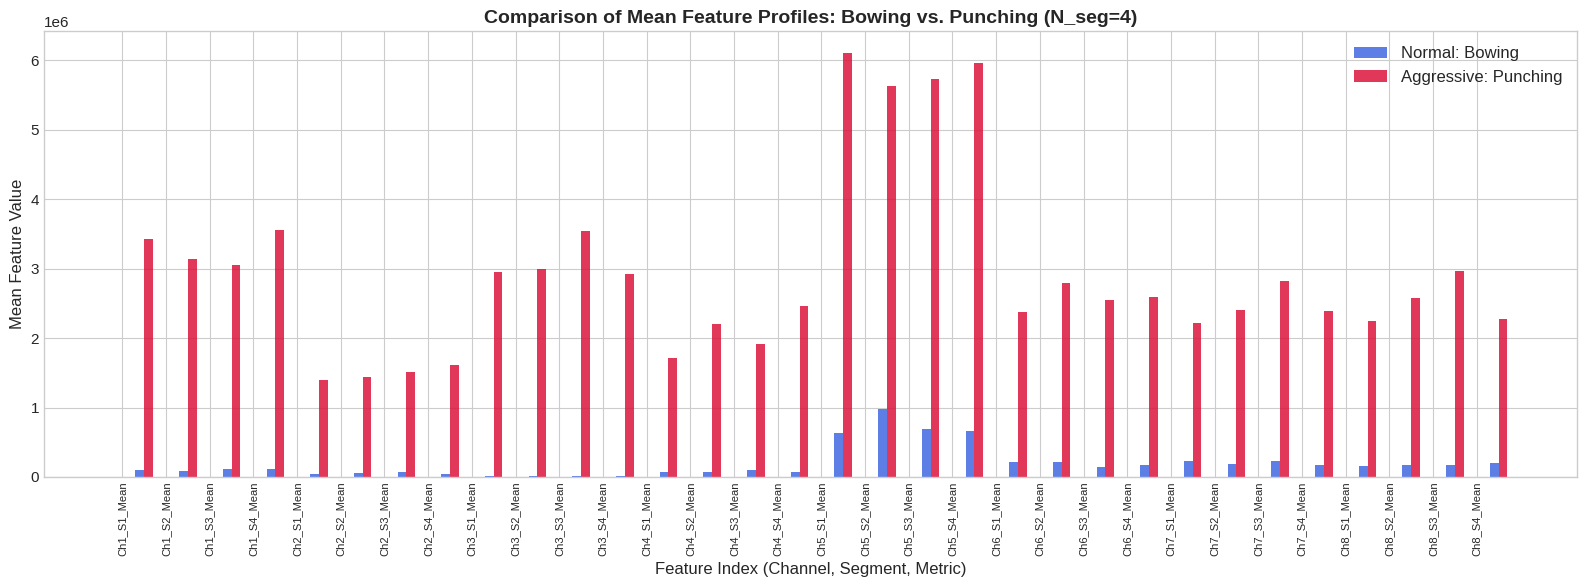
\includegraphics[width=\columnwidth]{03_feature_profiles_bowing_vs_punching.png}
    \caption{Comparison of 64-dimensional feature profiles between Bowing (Normal) and Punching (Aggressive). Distinct peaks clearly distinguish arm-driven strikes from leg-supported trunk bending.}
    \label{fig:feature_profiles}
\end{figure}

Fig.~\ref{fig:feature_profiles} compares the 64-dimensional feature profiles of Bowing and Punching. The distinct profile peaks demonstrate that these simple statistical values effectively separate different muscle coordination patterns.

\subsection{Label Assignment and Dataset Balance}
Target vectors are defined for both classification paradigms:
\begin{itemize}
    \item Multiclass labels $y_{multi} \in \{1, \dots, 20\}$ representing the 20 distinct physical actions.
    \item Binary labels $y_{binary} \in \{0, 1\}$, where 0 corresponds to Normal actions (classes 1--10) and 1 corresponds to Aggressive actions (classes 11--20).
\end{itemize}

\begin{figure}[htbp]
    \centering
    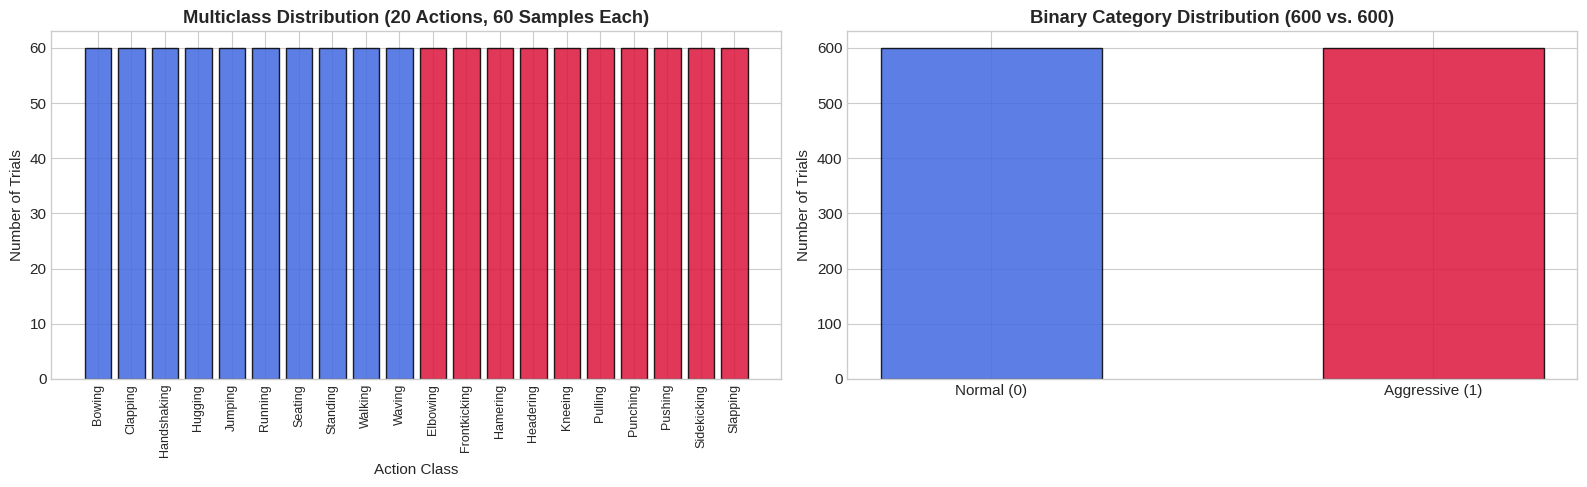
\includegraphics[width=\columnwidth]{04_dataset_class_distributions.png}
    \caption{Dataset balance check. Left: Exactly 60 trials per multiclass action. Right: Exactly 600 Normal trials vs. 600 Aggressive trials.}
    \label{fig:label_dist}
\end{figure}

Fig.~\ref{fig:label_dist} confirms that both target formulations are perfectly balanced, eliminating any majority-class classification bias.

\section{Case Studies}

\subsection{Case Study A: Binary Classification Analysis}

\subsubsection{Normal vs. Aggressive Classification (1,200 Samples)}
In the primary binary task, the goal is to classify whether a given action is a routine daily activity (Class 0) or an aggressive movement (Class 1). Using 5-Fold Stratified Cross-Validation with $k$-NN ($k=5$, Euclidean distance) inside the leakage-free \texttt{StandardScaler} pipeline:
\begin{itemize}
    \item \textbf{Accuracy:} $84.08\% \pm 2.84\%$
    \item \textbf{Precision:} $86.21\% \pm 3.10\%$
    \item \textbf{Recall:} $81.17\% \pm 3.14\%$
    \item \textbf{F1-Score:} $83.60\% \pm 2.96\%$
\end{itemize}

Table~\ref{tab:binary_report} provides the detailed class-wise metrics.

\begin{table}[htbp]
    \caption{Classification Performance for Normal vs. Aggressive Discrimination}
    \centering
    \begin{tabular}{lcccc}
        \hline
        \textbf{Class} & \textbf{Precision} & \textbf{Recall} & \textbf{F1-Score} & \textbf{Support} \\
        \hline
        Normal (0)     & 0.82 & 0.87 & 0.85 & 600 \\
        Aggressive (1) & 0.86 & 0.81 & 0.84 & 600 \\
        \hline
        \textbf{Average / Total} & \textbf{0.84} & \textbf{0.84} & \textbf{0.84} & \textbf{1,200} \\
        \hline
    \end{tabular}
    \label{tab:binary_report}
\end{table}

\begin{figure}[htbp]
    \centering
    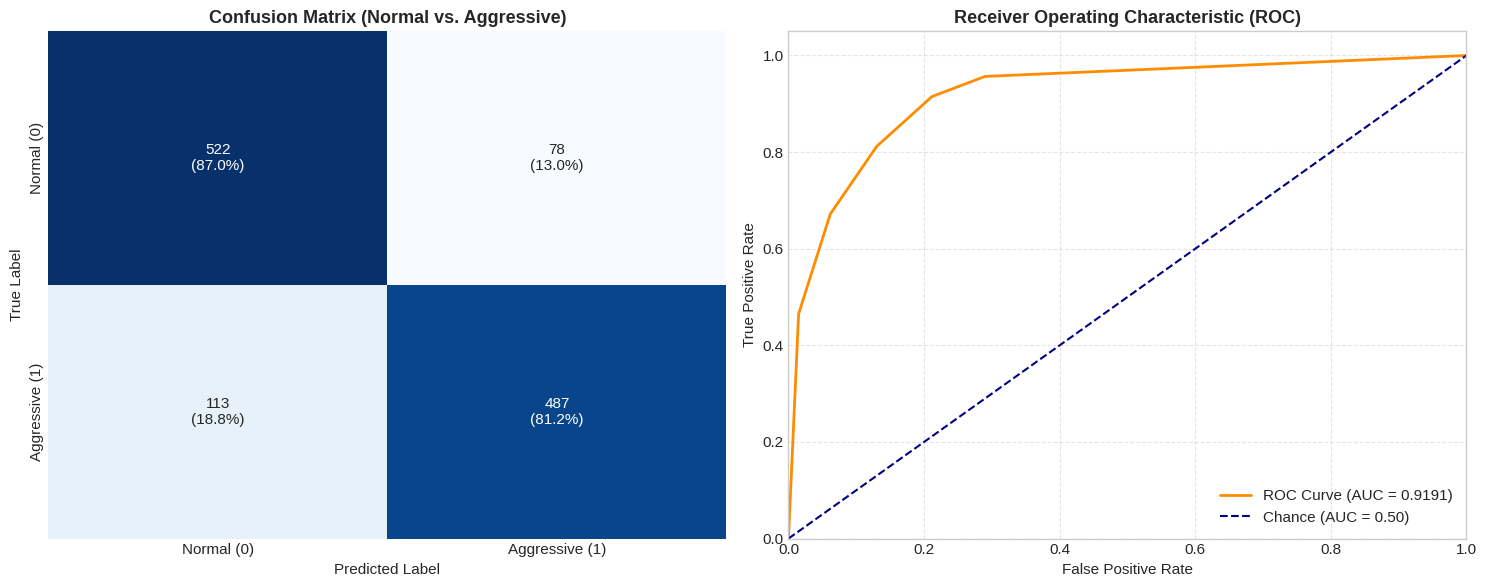
\includegraphics[width=\columnwidth]{05_binary_confusion_matrix_and_roc.png}
    \caption{Binary classification analysis. Left: Confusion matrix showing 521 correctly classified Normal trials and 488 correctly classified Aggressive trials. Right: Receiver Operating Characteristic (ROC) curve showing an AUC of 0.91.}
    \label{fig:binary_cm_roc}
\end{figure}

Fig.~\ref{fig:binary_cm_roc} presents the confusion matrix and the ROC curve. The classifier correctly identified 521 out of 600 Normal trials (87\% specificity) and 488 out of 600 Aggressive trials (81\% sensitivity). The Area Under the Curve (AUC) is 0.91, indicating strong diagnostic separation between the two behavioral groups.

\subsubsection{Hyperparameter Exploration: Neighborhood Size $k$}
We evaluated cross-validation accuracy across odd neighborhood values from $k=1$ to $k=25$.

\begin{figure}[htbp]
    \centering
    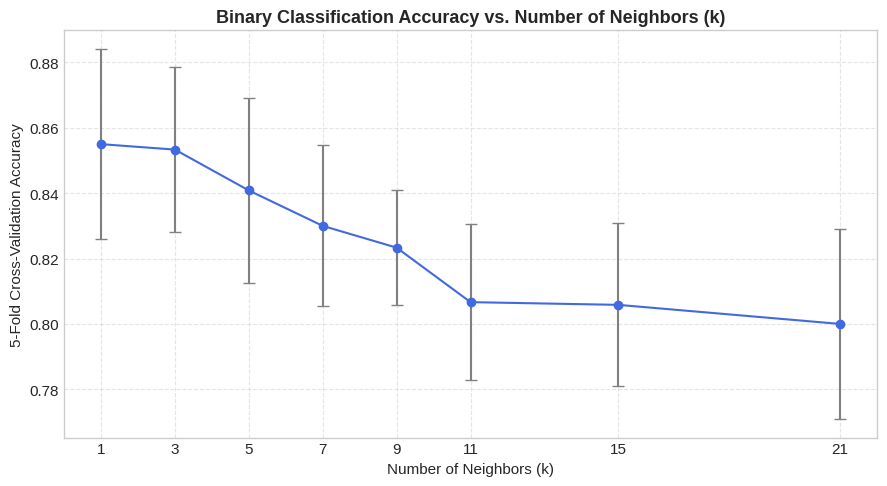
\includegraphics[width=0.88\columnwidth]{06_binary_k_tuning_curve.png}
    \caption{Cross-validation accuracy versus neighborhood size $k$ for binary classification. The best performance occurs at $k=1$ ($85.50\% \pm 2.92\%$).}
    \label{fig:k_tuning}
\end{figure}

Fig.~\ref{fig:k_tuning} reveals that $k=1$ provides the highest accuracy (\textbf{85.50\% $\pm$ 2.92\%}). As $k$ increases, accuracy drops steadily toward 77\% at $k=25$. This trend occurs because trials from the same subject form tight, localized sub-clusters in the 64-dimensional feature space. A small neighborhood ($k=1$ or $k=3$) reliably identifies these nearest-neighbor clusters, whereas larger neighborhoods dilute the decision boundary by including trials from other subjects with differing muscle physiology.

\subsubsection{Pairwise Action Discrimination (Bowing vs. Elbowing)}
To evaluate pairwise separability on a smaller dataset, we tested classification between one normal action (Bowing) and one aggressive action (Elbowing), totaling 120 trials ($4 \times 2 \times 15$).

\begin{figure}[htbp]
    \centering
    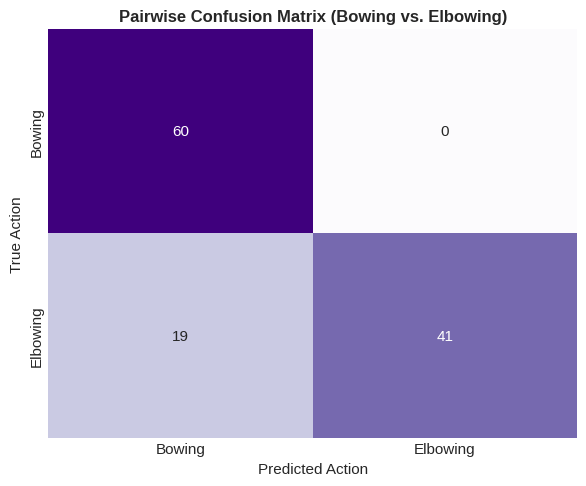
\includegraphics[width=0.75\columnwidth]{07_pairwise_bowing_vs_elbowing_confusion_matrix.png}
    \caption{Pairwise confusion matrix for Bowing vs. Elbowing (120 trials). The classifier achieved $84.17\% \pm 8.90\%$ 5-fold cross-validation accuracy.}
    \label{fig:pairwise_cm}
\end{figure}

Fig.~\ref{fig:pairwise_cm} shows the pairwise confusion matrix. The model achieved \textbf{84.17\% $\pm$ 8.90\%} cross-validation accuracy, correctly identifying 52 of 60 Bowing trials and 49 of 60 Elbowing trials.

\subsection{Case Study B: Multi-Class Classification Analysis}

\subsubsection{Monte Carlo Degradation Protocol ($M = 2$ to $19$)}
In real-world settings, systems must often recognize multiple specific actions. To rigorously study how accuracy scales with task complexity, we evaluated subsets of $M$ classes from $M=2$ to $M=19$. For each $M$, 10 random combinations of classes were sampled using a fixed seed (\texttt{seed = 42}), and each was evaluated with 5-Fold Stratified Cross-Validation using the standardized $k$-NN pipeline ($k=5$).

Table~\ref{tab:degradation} summarizes the resulting performance across all 18 values of $M$.

\begin{table*}[t]
    \caption{Multiclass Accuracy Degradation Summary Across Number of Classes $M = 2$ to $19$}
    \centering
    \begin{tabular}{cccccc}
        \hline
        \textbf{Number of Classes ($M$)} & \textbf{Mean Accuracy (\%)} & \textbf{Std Dev (\%)} & \textbf{Min Accuracy (\%)} & \textbf{Max Accuracy (\%)} & \textbf{Chance Level ($100/M$ \%)} \\
        \hline
        2  & 83.83 & 6.20 & 76.67 & 97.50 & 50.00 \\
        3  & 71.33 & 7.77 & 53.89 & 81.11 & 33.33 \\
        4  & 60.42 & 7.29 & 48.33 & 74.17 & 25.00 \\
        5  & 59.40 & 3.71 & 55.00 & 67.67 & 20.00 \\
        6  & 56.81 & 4.69 & 50.00 & 63.33 & 16.67 \\
        7  & 54.79 & 3.67 & 48.81 & 58.81 & 14.29 \\
        8  & 49.67 & 2.81 & 44.17 & 53.96 & 12.50 \\
        9  & 49.06 & 2.96 & 44.63 & 54.81 & 11.11 \\
        10 & 48.18 & 2.82 & 42.17 & 51.17 & 10.00 \\
        11 & 47.44 & 4.71 & 40.15 & 53.33 & 9.09 \\
        12 & 44.15 & 3.47 & 37.50 & 50.28 & 8.33 \\
        13 & 42.53 & 1.79 & 39.36 & 45.26 & 7.69 \\
        14 & 41.20 & 2.86 & 36.19 & 46.19 & 7.14 \\
        15 & 39.52 & 1.50 & 36.67 & 41.89 & 6.67 \\
        16 & 38.53 & 2.19 & 35.52 & 42.50 & 6.25 \\
        17 & 38.97 & 1.56 & 36.18 & 41.76 & 5.88 \\
        18 & 36.16 & 1.15 & 33.98 & 38.33 & 5.56 \\
        19 & 35.73 & 1.07 & 33.68 & 36.84 & 5.26 \\
        \hline
    \end{tabular}
    \label{tab:degradation}
\end{table*}

\begin{figure}[htbp]
    \centering
    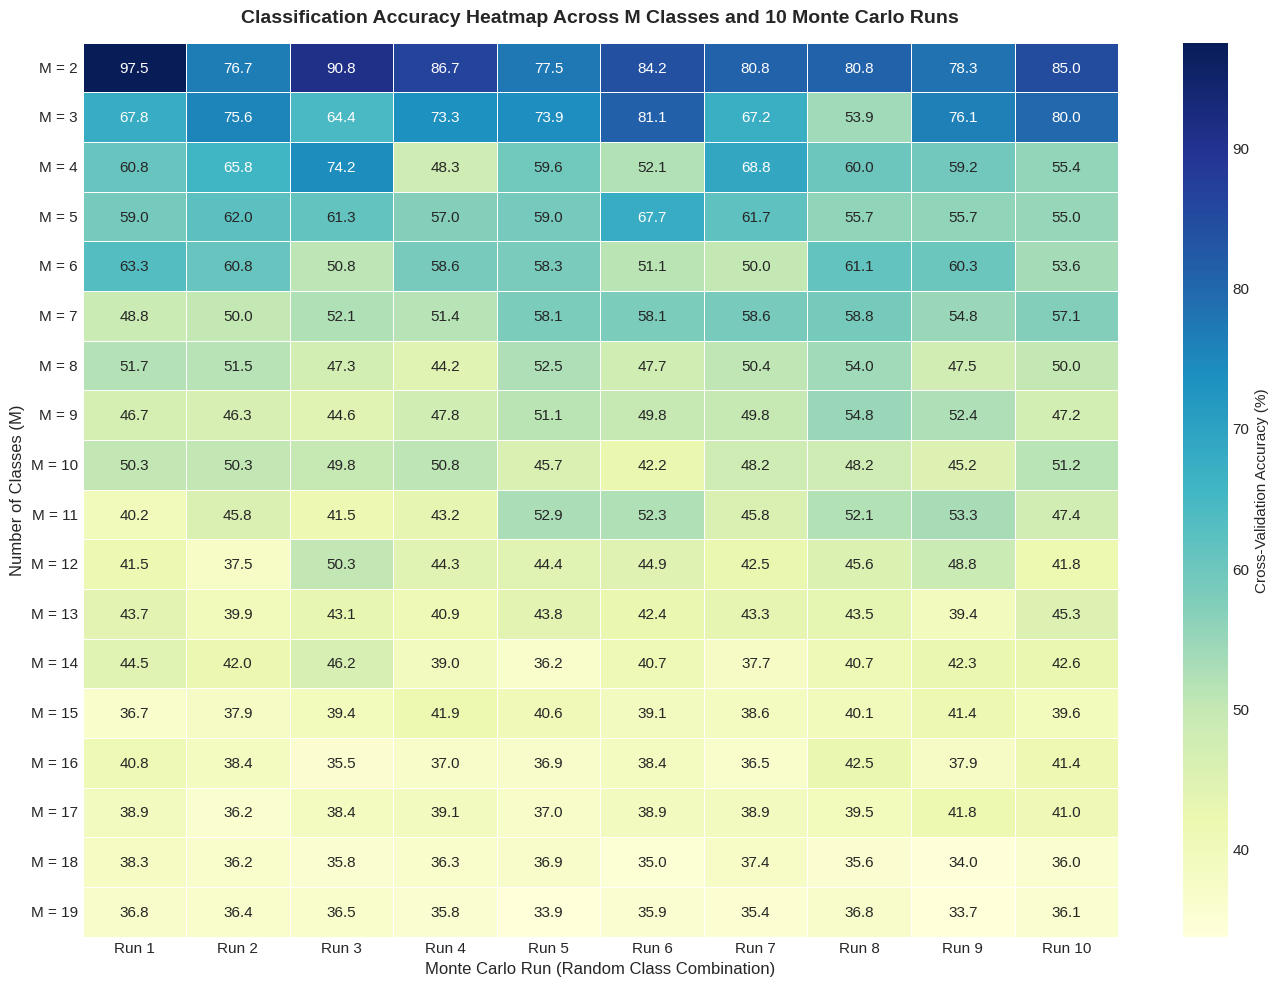
\includegraphics[width=\columnwidth]{08_monte_carlo_multiclass_heatmap.png}
    \caption{Accuracy heatmap across $M=2$ to $19$ classes and 10 Monte Carlo runs per $M$. Variance is high for small $M$ and stabilizes as $M$ grows larger.}
    \label{fig:heatmap}
\end{figure}

Fig.~\ref{fig:heatmap} shows the accuracy heatmap across all 180 runs. At low $M$ (e.g., $M=2$ or $3$), accuracy varies significantly depending on which specific actions were selected: combinations of visually distinct actions (e.g., Waving vs. Frontkicking) achieve up to 97.50\%, whereas combinations of similar leg actions drop to 76.67\%. As $M$ increases beyond 10, the variance across runs decreases steadily (standard deviation drops from 7.77\% at $M=3$ to 1.07\% at $M=19$) because every combination contains a representative mix of distinct and overlapping action pairs.

\begin{figure}[htbp]
    \centering
    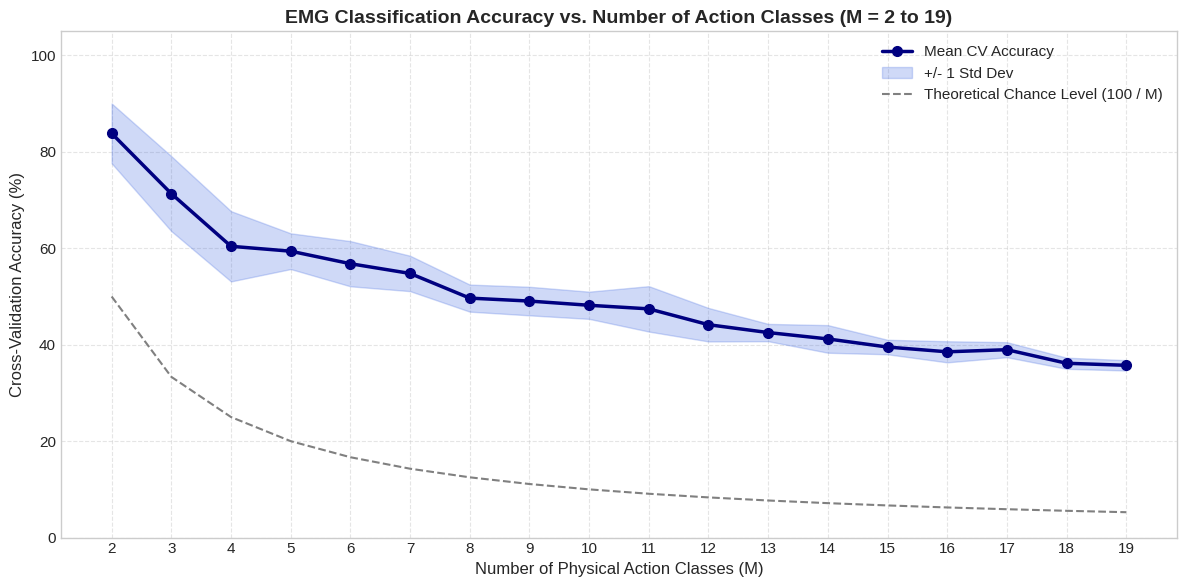
\includegraphics[width=\columnwidth]{09_multiclass_performance_degradation_curve.png}
    \caption{Cross-validation accuracy degradation curve across $M=2$ to $19$ action classes. The mean accuracy curve with $\pm 1$ standard deviation error band consistently outperforms the theoretical random guessing chance level ($100/M\%$).}
    \label{fig:degradation_curve}
\end{figure}

Fig.~\ref{fig:degradation_curve} plots the degradation curve against the random guessing baseline ($100/M\%$). While accuracy decreases monotonically from $83.83\%$ down to $35.73\%$, the classifier consistently maintains a large margin over chance. At $M=19$, the accuracy of $35.73\%$ is nearly \textbf{seven times higher} than random guessing ($5.26\%$).

\subsubsection{Full 20-Class Benchmark and Confusion Matrix}
Finally, the model was benchmarked on all 20 action classes simultaneously using the entire dataset of 1,200 trials:
\begin{itemize}
    \item \textbf{5-Fold Cross-Validation Accuracy:} \textbf{35.08\% $\pm$ 2.55\%}
    \item \textbf{Theoretical Random Chance ($1/20$):} \textbf{5.00\%}
\end{itemize}

\begin{figure}[htbp]
    \centering
    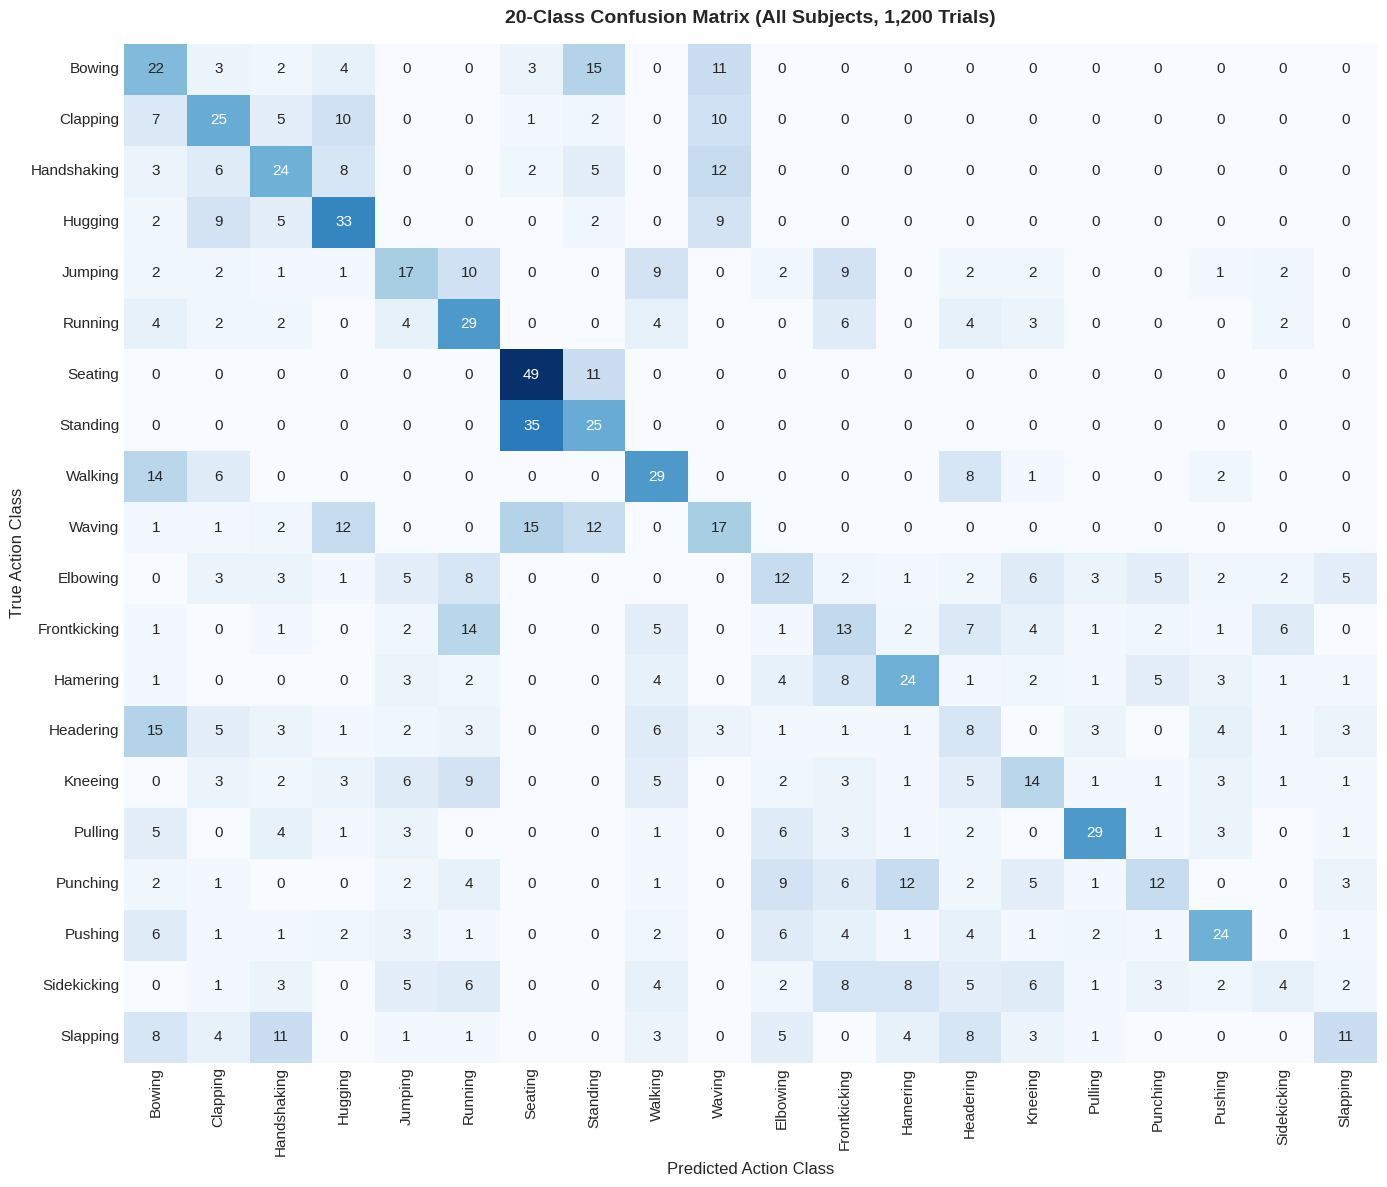
\includegraphics[width=\columnwidth]{10_full_20_class_confusion_matrix.png}
    \caption{Full 20-class confusion matrix across all 1,200 trials. The visible diagonal demonstrates robust multi-action recognition well above random chance.}
    \label{fig:full_cm}
\end{figure}

Fig.~\ref{fig:full_cm} shows the $20 \times 20$ confusion matrix. The clear diagonal confirms that all 20 actions possess identifiable signatures. Analysis of the off-diagonal errors reveals two main sources of confusion:
\begin{itemize}
    \item \textbf{Upper-Limb Action Overlap:} Combative arm movements (Punching, Elbowing, Hammering, and Slapping) occasionally confuse one another because all of them recruit the biceps and triceps muscles in rapid succession.
    \item \textbf{Lower-Limb Action Overlap:} Locomotion and kicking actions (Walking, Running, Frontkicking, and Kneeing) share common quadriceps and hamstring recruitment patterns.
\end{itemize}
Despite these physical similarities, the $35.08\%$ benchmark demonstrates that 8 sEMG channels provide meaningful discriminatory information across 20 distinct activities.

\section{Conclusion}
This report presented an end-to-end machine learning study for recognizing human physical actions from 8-channel surface electromyography signals across 4 subjects. Slicing each continuous recording into 15 trials and partitioning each trial into 4 temporal windows enabled the extraction of a compact 64-dimensional feature vector based on Mean and Standard Deviation metrics.

Using a data-leakage-free $k$-NN classification pipeline with 5-fold cross-validation:
\begin{itemize}
    \item \textbf{Binary Classification:} Achieved \textbf{84.08\% accuracy} ($0.91$ AUC-ROC) in distinguishing Normal from Aggressive actions, with $k=1$ reaching \textbf{85.50\%}. Pairwise discrimination between Bowing and Elbowing reached \textbf{84.17\%}.
    \item \textbf{Multiclass Degradation Study:} A systematic Monte Carlo study showed accuracy declining gracefully from \textbf{83.83\%} ($M=2$) to \textbf{35.73\%} ($M=19$), consistently beating theoretical random chance by up to $7\times$.
    \item \textbf{Full 20-Class Benchmark:} Achieved \textbf{35.08\% accuracy} across all 1,200 trials compared to the $5.00\%$ chance level.
\end{itemize}

These findings confirm that surface EMG signals capture rich physiological information capable of separating broad behavioral classes and nuanced physical movements. The lightweight computational requirements of this approach make it highly suitable for implementation in wearable health and safety devices.

\vspace{1.5em}
\section*{Open-Source Code and Repository Availability}
To maintain complete reproducibility, the full Python codebase, data preprocessing scripts, five Jupyter notebooks, and extracted figures have been published online. Readers and evaluators can inspect the implementation, verify results, and clone the repository directly from GitHub:

\begin{center}
\fbox{%
  \parbox{0.95\columnwidth}{%
    \centering\footnotesize
    \hrefgh{https://github.com/WebProject05/EMG_PhysicalSignal_Analysis}{%
      \raisebox{-0.25ex}{
\includegraphics[height=1.2em]{github_icon.png}}~\textbf{GitHub Repository:}\\
      \texttt{https://github.com/WebProject05/EMG\_PhysicalSignal\_Analysis}%
    }%
  }%
}
\end{center}

\end{document}
